\chapter{Architecture}

This chapter describes the architecture of JPaxos.
First the general architecture of the library is presented, consecutively focusing on its parts in detail.
Later the most significant data structures and the threading architecture details are presented.

\section{Architecture overview}
\indent\par
The easiest way to understand the architecture of JPaxos is to analyze its architecture in top-down approach.

\subsection{Processes and their communication}

From the perspective of JPaxos library user, we can distinguish two types of processes -- replicas and clients. The replica process is responsible for state machine replication. This process receives commands (requests) from clients, executes them on state machine in the same order on every replica, and sends the results (of commands execution) back to clients. The client process sends commands to replicated service (replicas) and waits for the results. 

The user of JPaxos library has to provide implementation of a service (that executes clients requests and generates responses) and a client application that generates requests to service and waits for responses.

The JPaxos library provides two modules used to replicate a service:
\begin{tightList}
  \item[\textbf{JPaxos Replica}] - module of JPaxos library responsible for global request ordering, passing the requests to the service, answering to the clients and recovering service from crash.
  \item[\textbf{JPaxos Client}] - module of JPaxos responsible for connecting and sending commands to JPaxos Replica module. It also handles crashes of replicas, and ensures that the request will be eventually executed on replicated service
\end{tightList}

There are two possible approaches of building replicated services using JPaxos.
The first, recommended by us, is to integrates the JPaxos \texttt{Client}
module with client application.  This approach provides full transparency of
replication for the clients. The service client contacts with the JPaxos
\texttt{Client} module as if it would contact the service, i.e. it executes
requests and gets answers for them. This approach is presented on figure
\ref{fig:jpaxos_processes}a. 

\begin{figure}[h]
 \begin{tabular}{ccc}
  
\includegraphics[width=0.45\textwidth]{architecture/userArchitecture1.pdf}
  &
  \hspace{0.01\textwidth}
  &
  
\includegraphics[width=0.45\textwidth]{architecture/userArchitecture2.pdf}
  \\ 
  \scriptsize a) JPaxos client integrated with service client
  & & 
  \scriptsize b) JPaxos client integrated with the replica\\
 \end{tabular}
 \caption{Two models of JPaxos}\label{fig:jpaxos_processes}
\end{figure}

The other approach incorporates the JPaxos \texttt{Client} module within
replica. Because the client application is not using JPaxos \texttt{Client}
module any more, the transparency is lost, and the programmer must
take care of selecting a working (not crashed) replica himself. However, this
approach enables using JPaxos in a wider context. For example, one could
possibly create a REST web service, and use a usual web client as the service
client, while the service itself would be replicated using JPaxos.  This
approach is visualised in figure \ref{fig:jpaxos_processes}b.


The service itself must be integrated within JPaxos \texttt{Replica} module. Service gets the requests and returns the response. However, in order to make the resource usage bounded, JPaxos requires snapshotting functionality from the service (described in section \ref{sec:snapshotting})
what partially breaks transparency. 

\subsection{Client and client-replica communication}

The JPaxos client module is a single, light-weight module that performs several tasks:

\begin{tightList}[\setlength{\topsep}{0pt} \setlength{\partopsep}{0pt}]
 \item[\textbullet] Connects to the replicated service
 \item[\textbullet] Reconnects automatically to the replicated service if the connection is lost
 \item[\textbullet] Retrieves (or acknowledges) a client ID for recognising the requests
 \item[\textbullet] Sends the requests
 \item[\textbullet] Waits for answer, retransmitting the request if needed
\end{tightList}

\noindent For the communication with replicas, the client module uses TCP protocol.

\subsection{Service}

% TODO TZ More information about service, service proxy, service interface, service module
% TODO TZ move ServiceProxy section here

The Service module is the core part -- in fact it is the service that uses JPaxos for replication.
In order to integrate a service with the library, it must implement an interface specified in JPaxos. The interface provides required communication between the library and the service.

The interface for interconnecting JPaxos replica and service allows for:
\begin{tightList}
 \item[\textbullet] Executing requests and providing answers for them
 \item[\textbullet] Creating snapshots
 \item[\textbullet] Recovering from snapshots
\end{tightList}

\subsection{Replica}

Replica is the most important part of JPaxos. It consists of numerous modules as depicted in figure \ref{fig:replica_architecture}.

\begin{figure}[h]
 \centering
 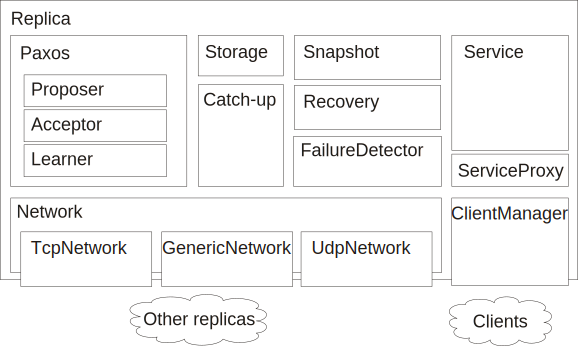
\includegraphics[keepaspectratio, width=0.75\textwidth]{architecture/replica_architecture.pdf}
 \caption{Block diagram of JPaxos modules}
 \label{fig:replica_architecture}
\end{figure}

Short description of the JPaxos modules goes as follows:

\begin{description}
  \item[Replica ] interconnects other modules -- especially the ClientManager, Paxos ans ServiceProxy
  \item[ClientManager ] maintains connection to clients, receives requests from them and forwards the answers
  \item[Paxos ] implements the MultiPaxos consensus algorithm
  \begin{description}
    \item[Proposer ] sends new proposes
    \item[Acceptor ] receives proposes and accepts them
    \item[Learner ] collects accepts and decides
  \end{description}
  \item[CatchUp ] takes care for lost ballots and retrieves the state from others on recovery
  \item[SnapshotMaintainer ] controls the snapshot mechanism
  \item[Recovery ] chooses a proper recovery method and does the actual recovery processes
  \item[Storage ] keeps the state of the Paxos protocol, i.e. view number, log of consensus instances and a snapshot
  \item[Service Proxy ] contacts with the user defined Service, provides as much trans\-pa\-rency as possible for the service
\end{description}

\section{Storage and data structures}
\label{sec:storage_and_data_structures}

Apart of modules and interaction among them it is important to design proper routines for accessing the data.
One should choose proper way of storing the data used in a single module, but much more challenging is to design proper structures and access methods for the data shared across JPaxos. Below we describe how we store the most significant data in our library.

\subsection{Process descriptor}

Every application has some configurable options that stay unchanged during the run. In JPaxos all these constants are kept in the \texttt{ProcessDescriptor} class.

During the system startup, JPaxos reads a configuration file and initializes \texttt{ProcessDescriptor} with proper values for:
\begin{tightList}[\setlength{\labelwidth}{0em}]
 \item[\textbf{crashModel}] the crash model (see chapter \ref{chapter:recovery})
 \item[\textbf{logPath}] path for the stable storage
 \item[\textbf{localId}] the identification number of the replica
 \item[\textbf{numReplicas}] count of the replicas
 \item[\textbf{windowSize}] a preferred window size (see \ref{subsec:concurrent_instances})
 \item[\textbf{batchingLevel}] a maximum size of the batch (see \ref{sec:batching})
 \item[\textbf{maxBatchDelay}] delay for connecting requests for batching in milliseconds
 \item[\textbf{network}] network protocol to be used (TCP or UDP)
 \item[\textbf{maxUdpPacketSize}] a maximum size of UDP-datagram sent by GenericNetwork
\end{tightList}

\subsection{Storage interface}
\label{subsec:storage_interface}

\texttt{Storage} interface is responsible for holding state of the Paxos protocol.

The state of Paxos is shared across various modules.
It is very likely that various threads might want to access the \texttt{Storage} simultaneously. In order to prevent concurrency-related errors only one thread, the Dispatcher (see section \ref{sec:threads}), may access these data. 

\paragraph{\normalfont \ttfamily Storage}
holds the data as follows:
\begin{tightList}[\setlength{\labelwidth}{0em}]
  \item[\textbf{log}] the Paxos Log (see section \ref{subsec:the_paxos_log})
  \item[\textbf{view}] current view
  \item[\textbf{firstUncommitted}] first instance not decided yet
  \item[\textbf{windowSize}] the current size of the window used for multiple instances
  \item[\textbf{acceptors}] a list of processes acting as acceptors
  \item[\textbf{snapshot}] the most recent snapshot (see section \ref{sec:snapshotting})
  \item[\textbf{epoch}] the current epoch vector (see section \ref{sec:epoch_ss})
\end{tightList}

\strut

The type of \texttt{Storage} implementation must be chosen according to requirements imposed by the model or recovery.
The implementation decides which elements must be kept in the stable storage and which may be placed in volatile memory.

\subsection{The Paxos Log}
\label{subsec:the_paxos_log}

The most important data structure for Paxos, the Log, is part of the \texttt{Storage}.
In our program responsible for storing list of Paxos instances is the \texttt{Log} interface and the \texttt{Con\-sen\-susInstance} class.

\texttt{ConsensusInstance} is a class keeping information about single instance of Paxos and contains:

\begin{tightList}[\setlength{\itemindent}{0pt}\setlength{\leftmargin}{2\leftmargin}]
  \item[\textbf{view}] a view of the last received message related with this instance,
  \item[\textbf{value}] the value which is held by this instance (i.e. packed requests that are received from clients and executed when the state is set to DECIDED), 
  \item[\textbf{state}] the instance can be in one of three states:
  \begin{tightList}[\setlength{\itemindent}{0pt} \setlength{\labelwidth}{7em}]
    \item[\texttt{\tiny UNKNOWN}] no information about the value of this instance,
    \item[\texttt{\tiny KNOWN}] a view and value are specified and \textbf{can} be changed later,
    \item[\texttt{\tiny DECIDED}] a value is already chosen and \textbf{cannot} be changed.
  \end{tightList}
  \item[\textbf{accepts}] set of known replicas which accepted the (view, value) pair.
\end{tightList}

Theoretically \texttt{Log} should contain all instances from the first up to the current one.
Of course such data structure cannot be implemented. The log must be bounded, however it must contain all instances that are still needed. The question is which instances are still needed and which may be truncated.

Without the snapshotting (see \ref{sec:snapshotting}) every instance must be kept in log. With snapshotting only the instances since the last snapshot are needed. The instance with lowest ID that is still needed is the first instance that should be executed after updating the service state to the state from the last snapshot. This instance is the lowest instance that always is present in the log -- therefore we call it the lowest availabile one. The \textit{lowestAvailableId} is the ID of this instance.

The smallest yet unused instance ID is called by us the \textit{nextId}, as it will be the ID assigned to the next instance.

The \texttt{Log} implementation always keeps all instances with ID between \textit{lowestAvailableId} (inclusive) and \textit{nextId} (exclusive). Instances below \textit{lowestAvailableId} have already been truncated and instances above \textit{nextId} are yet unknown.

Appending, retrieving and truncating instances are three main operations per\-for\-med by log.

New instance can always be appended to the log and after this operation \textit{nextId} value is increased by 1. 

\noindent There are three possible cases of retrieving an instance with a specified \textit{id}:
\begin{tightList}
  \item[\textbullet] (\textit{id} $<$ \textit{lowestAvailableId}) -- instance has been truncated and null value is returned,
  \item[\textbullet] (\textit{lowestAvailableId} $\leq$ \textit{id} $<$ \textit{nextId}) -- instance is inside log so it is returned,
  \item[\textbullet] (\textit{nextId} $\leq$ \textit{id}) -- empty instances between \textit{nextId} and \textit{id} are created and the empty instance with ID \textit{id} is returned.
\end{tightList}

\noindent Old instances can be removed by snapshotting only. When the replica receives a new snapshots, the log is truncated and the \textit{lowestAvailableId} is increased.

\section{Threading Model}
\label{sec:threads}

Multi-threaded applications are very often complex, hard to debug and test. But single threaded applications cannot fully utilise multi-core processors. The JPaxos library is using multiple threads, but every variable in the library can be accessed only from one thread, what decreases the complexity and makes the code easier to test and maintain.

We can divide threads in JPaxos library into two categories - task based and
network related. 
Task based thread provides a method to add new tasks (work
items) to the queue . When the queue is not empty, the thread takes the task
with highest priority and executes it. If no task is available, the thread is
sleeping. The network related threads are used to receive and send messages
over the network.

Below we describe the threads in JPaxos, their responsibilities and interactions between them. 

\begin{description}
  \item[Replica thread] \hfill

    The replica thread is task based thread. New tasks are scheduled upon a signal from Paxos about a new decision, or when new snapshot was received or made by service. For most of the time this thread waits for new decided consensus instances. When new request is decided by Paxos, it is executed by service in replica thread. Also all snapshot related tasks are executed in this thread. Other threads (e.g. Paxos dispatcher) may therefore safely execute their snapshot-concerning routines.
    
  \item[Paxos dispatcher] \hfill \nopagebreak
    
    This is also task based thread. It executes tasks related to Paxos consensus algorithm as well as provides secure access to critical data structures -- to the \texttt{Storage} (see subsection \ref{subsec:storage_interface}). This thread is also responsible for sending, receiving and handling most of protocol messages as well as accessing the \texttt{Storage} and triggering catch-Up. All tasks are prioritized, so for example, writes to the storage and the Paxos-related processing events have a higher priority than the catch-Up tasks.
    
    New tasks are added in the following situations:
    \begin{tightList}
      \item[\textbullet] a new message has been received - related message handler is executed
      \item[\textbullet] a new message has been sent
      \item[\textbullet] failure detector suspects the leader
      \item[\textbullet] failure detector should sent \alive message
      \item[\textbullet] proposer starts new proposal
      \item[\textbullet] message should be retransmitted
      \item[\textbullet] new snapshot is received (from service or catch-up)
      \item[\textbullet] a periodical catch-up should occur
    \end{tightList}
    
  \item[NioClientManager] \hfill

    This is thread used to handle connections with clients. By using java.nio package, we only need one thread to manage all clients connection. Every time a new event occurs (an incoming connection waits for accepting, data received from client, data ready to be sent) an appropriate action is executed. 

  \item[UdpNetwork] \hfill

    This thread is responsible for listening on DatagramSocket for incoming UDP datagram packages. Every time a new message is received, it is deserialised and all listeners are notified.

  \item[TcpNetwork] \hfill

    For TCP connection between each two replicas a separate thread for receiving and transmitting is created. Also there is one thread which waits for new incoming connections. Overall, we have $n-1$ threads for receiving data from $n-1$ other replicas, $n-1$ threads for transmitting data and 1 thread for new incoming connection. It gives $(n - 1) + (n - 1) + 1 = 2 \cdot n - 1$ threads handling TCP. Each receiving and transmitting thread can be in one of three states:
    \begin{itemize}
            \item connected, waiting for new messages,
            \item not connected, trying to establish a new connection,
            \item waiting for a new connection to be established by other replica.
    \end{itemize}
\end{description}
